\documentclass[11pt]{article}
% ------------------------------------------------------------------
% The Tiny Language Model: a lecture narrative on the transformer
% Companion to Labs/10.Transformer/tutorial_tiny_language_model_ABC.ipynb
% Build: latexmk -pdf tlm_transformer_narrative.tex
% ------------------------------------------------------------------
\usepackage[utf8]{inputenc}
\IfFileExists{lmodern.sty}{\usepackage[T1]{fontenc}\usepackage{lmodern}}{}
\usepackage{microtype}
\usepackage[margin=2.6cm]{geometry}
\usepackage{amsmath,amssymb,bm}
\usepackage{booktabs,array,tabularx}
\usepackage{enumitem}
\usepackage{xcolor}
\usepackage{tikz}
\usetikzlibrary{positioning,fit,arrows.meta,shapes.geometric,calc,backgrounds}
\usepackage{caption}
\usepackage[colorlinks=true,linkcolor=blue!50!black,urlcolor=blue!50!black,citecolor=blue!50!black]{hyperref}

\setlist{itemsep=2pt,topsep=4pt}
\captionsetup{font=small,labelfont=bf}
\setlength{\parskip}{4pt}

% ---- notation ----------------------------------------------------
\newcommand{\tok}[1]{\texttt{<#1>}}
\newcommand{\code}[1]{\texttt{#1}}
\newcommand{\V}{\mathbb{V}}
\newcommand{\R}{\mathbb{R}}
\newcommand{\softmax}{\operatorname{softmax}}
\newcommand{\LN}{\operatorname{LN}}
\newcommand{\Etok}{E_{\text{tok}}}
\newcommand{\Epos}{E_{\text{pos}}}

% ---- colours and TikZ styles -------------------------------------
\definecolor{edge}{gray}{0.45}
\definecolor{accent}{RGB}{37,99,180}
\definecolor{tint}{gray}{0.93}
% block colours of the architecture figure (after Vaswani et al., 2017)
\definecolor{cEmb}{HTML}{FBE3E3}
\definecolor{cAtt}{HTML}{FCE3C4}
\definecolor{cNorm}{HTML}{F3F4C9}
\definecolor{cFF}{HTML}{CDEEF8}
\definecolor{cLin}{HTML}{DDDEF4}
\definecolor{cSoft}{HTML}{CFEBD5}
\definecolor{cMask}{HTML}{EDE7F6}
\tikzset{
  >={Stealth[length=2.2mm]},
  flow/.style={->,draw=edge,line width=0.7pt},
  blk/.style={draw=edge,rounded corners=4pt,align=left,inner sep=5pt,
              font=\small,fill=white,line width=0.6pt},
  hl/.style={blk,draw=accent,fill=accent!8,line width=1.2pt},
  note/.style={font=\footnotesize\color{black!60},align=left},
}

\title{\textbf{The Tiny Language Model}\\[2pt]
  \large A lecture narrative on the decoder-only transformer}
\author{Harrison B.\ Prosper\\[2pt]
  \small PHY 6937, \emph{Machine Learning in Physics}, Florida State University}
\date{October 2026}

\begin{document}
\maketitle

\begin{abstract}\noindent
This note accompanies the notebook \code{tutorial\_tiny\_language\_model\_ABC.ipynb}.
It explains, component by component, the decoder-only transformer built there:
a model with 136{,}169 parameters that learns to write the Taylor series, to
$\mathcal{O}(x^6)$, of functions such as $\cosh^3(ax)+\tanh(bx)$, one token at a
time. The emphasis is on what each component computes, the shapes of the tensors
it acts on, and how the trained network is used autoregressively to generate text.
\end{abstract}

\tableofcontents
\bigskip

% ==================================================================
\section{Overview}
% ==================================================================

The tiny language model (TLM) is a decoder-only transformer. Given a prompt such as
\code{cosh(a*x)**3 + tanh(b*x)}, it emits the Taylor series of the function to
$\mathcal{O}(x^6)$, one token at a time. With greedy decoding it reproduces, character
for character, the correct series for $99.3\% \pm 0.3\%$ of 800 held-out functions.

The whole model can be summarized in one sentence: \emph{integers become points in a
72-dimensional space; three times over, each point looks back at the points before
it and is then refined on its own; the final points are turned into a probability
distribution over the next token; the chosen token is appended, and the process
repeats.} Three ideas carry everything that follows.

\begin{description}[leftmargin=1.2em]
\item[Representation.] A sequence of $L$ tokens becomes a cloud of $L$ points in
  $\R^d$, with $d=72$. Each point encodes both \emph{what} the token is and
  \emph{where} it sits.
\item[Interaction.] Attention updates each point by a weighted average of (linearly
  transformed) points. The causal mask restricts the average to the point itself and
  the points before it.
\item[Generation.] The network answers only one question: \emph{what is the next
  token?} Long outputs come from feeding each answer back in as input.
\end{description}

\begin{table}[h]
\centering\small
\caption{Configuration of the model in the notebook.}
\label{tab:config}
\begin{tabular}{@{}llr@{}}
\toprule
Quantity & Symbol & Value \\
\midrule
Vocabulary size & $|\V|$ & 40 \\
Sequence length (padded) & $L_{\max}$ & 128 \\
Embedding dimension (\code{EMB\_DIM}) & $d$ & 72 \\
Decoder layers & $N$ & 3 \\
Attention heads per layer & $H$ & 8 \\
Head dimension, $d/H$ & $d_h$ & 9 \\
Feed-forward hidden width (\code{FF\_DIM}) & $d_{\text{ff}}$ & 128 \\
Dropout probability & & 0.1 \\
Trainable parameters & & 136{,}169 \\
Train / validation / test sequences & & 12{,}000 / 156 / 800 \\
Optimizer & & Adam, $8\times10^5$ iterations, batch 32 \\
Learning rate & & $1.6\times10^{-3}\to1.0\times10^{-4}$, 16 steps \\
\bottomrule
\end{tabular}
\end{table}

\paragraph{Notation.} Tensors carry the batch as their first index, as in the
Annotated Transformer. $B$ is the batch size and $L$ the length of the sequence being
processed. The notebook calls the embedding dimension both $d$ and $h$; here it is
always $d$.

% ==================================================================
\section{From text to integers}
% ==================================================================

Every training example is a single row of 128 integers: the prompt and its answer are
concatenated, not stored as a pair. This is the defining choice of a decoder-only
model. There is no separate encoder for the prompt; the prompt is simply the
beginning of the sequence the model learns to continue.

\subsection{Tokens and the vocabulary}

A regular-expression tokenizer splits each string into tokens, trying longer tokens
before shorter ones so that \code{sinh} is never read as \code{sin} followed by
\code{h}. The 40 distinct tokens are numbered as in Table~\ref{tab:vocab}.

\begin{table}[h]
\centering\small
\caption{The vocabulary $\V$.}
\label{tab:vocab}
\begin{tabularx}{\linewidth}{@{}lXX@{}}
\toprule
Codes & Tokens & Role \\
\midrule
0--3 & \tok{pad}, \tok{sos}, \tok{eos}, \tok{sep} & padding, start, end, prompt/answer separator \\
4--11 & space, \code{( ) * ** + - /} & punctuation and operators (\code{**} is one token) \\
12--21 & \code{0} \dots\ \code{9} & digits; the number 15 is two tokens \\
22 & \code{O(x**6)} & the whole error term is one token \\
23--39 & \code{a b c d f g h m n x}, \code{exp sin cos tan sinh cosh tanh} & symbols and function names \\
\bottomrule
\end{tabularx}
\end{table}

\subsection{One sequence, laid out}

The first sequence in the data file has the prompt \code{cosh(a*x)**3 + tanh(b*x)}.
Its layout by position is shown in Table~\ref{tab:layout}.

\begin{table}[h]
\centering\small
\caption{The first sequence of the data file, by position.}
\label{tab:layout}
\begin{tabular}{@{}lll@{}}
\toprule
Positions & Tokens & Codes \\
\midrule
0 & \tok{sos} & 1 \\
1--15 & \code{cosh ( a * x ) ** 3 + tanh ( b * x )} & \code{27 5 23 7 39 6 8 15 9 38 5 24 7 39 6} \\
16 & \tok{sep} & 3 \\
17--70 & \code{1 + b * x + \dots\ + O(x**6)} & \code{13 9 24 \dots\ 22} \\
71 & \tok{eos} & 2 \\
72--127 & \tok{pad} \dots\ \tok{pad} & \code{0 \dots\ 0} \\
\bottomrule
\end{tabular}
\end{table}

\noindent A sequence therefore has the general form
\begin{equation}
  \bm{X} = \tok{sos},\; p_1,\dots,p_m,\; \tok{sep},\; t_1,\dots,t_k,\; \tok{eos},\;
           \tok{pad},\dots,\tok{pad},
  \label{eq:layout}
\end{equation}
with $m=15$ prompt tokens and $k=54$ target tokens in this example. Two details
matter later.
\begin{itemize}
\item The \tok{eos} token immediately follows the last target token (position 71
  here), and the padding comes after it. The model therefore learns to end its output
  with \tok{eos}.
\item After filtering by length, the file holds 12{,}956 sequences of mean unpadded
  length 68.2 tokens (standard deviation 20.6), so on average about half of each row
  is padding.
\end{itemize}

An exhaustive search over outputs is hopeless: with $|\V|=40$ and $k\approx54$ there
are about $40^{54}\approx10^{86}$ candidate strings. The model must therefore be used
with a heuristic, here greedy decoding (Section~\ref{sec:generation}).

% ==================================================================
\section{The architecture at a glance}
% ==================================================================

Figure~\ref{fig:arch} shows the whole model. Read it top to bottom. The shape
$[B,L,72]$ is preserved from the embedding to the last layer normalization, so every
position carries its own 72-vector through the network. The two elbows on the left
are the residual (skip) paths, and the mask built from the token codes enters only
the attention block, the one place where positions exchange information.

\begin{figure}[p]
\centering
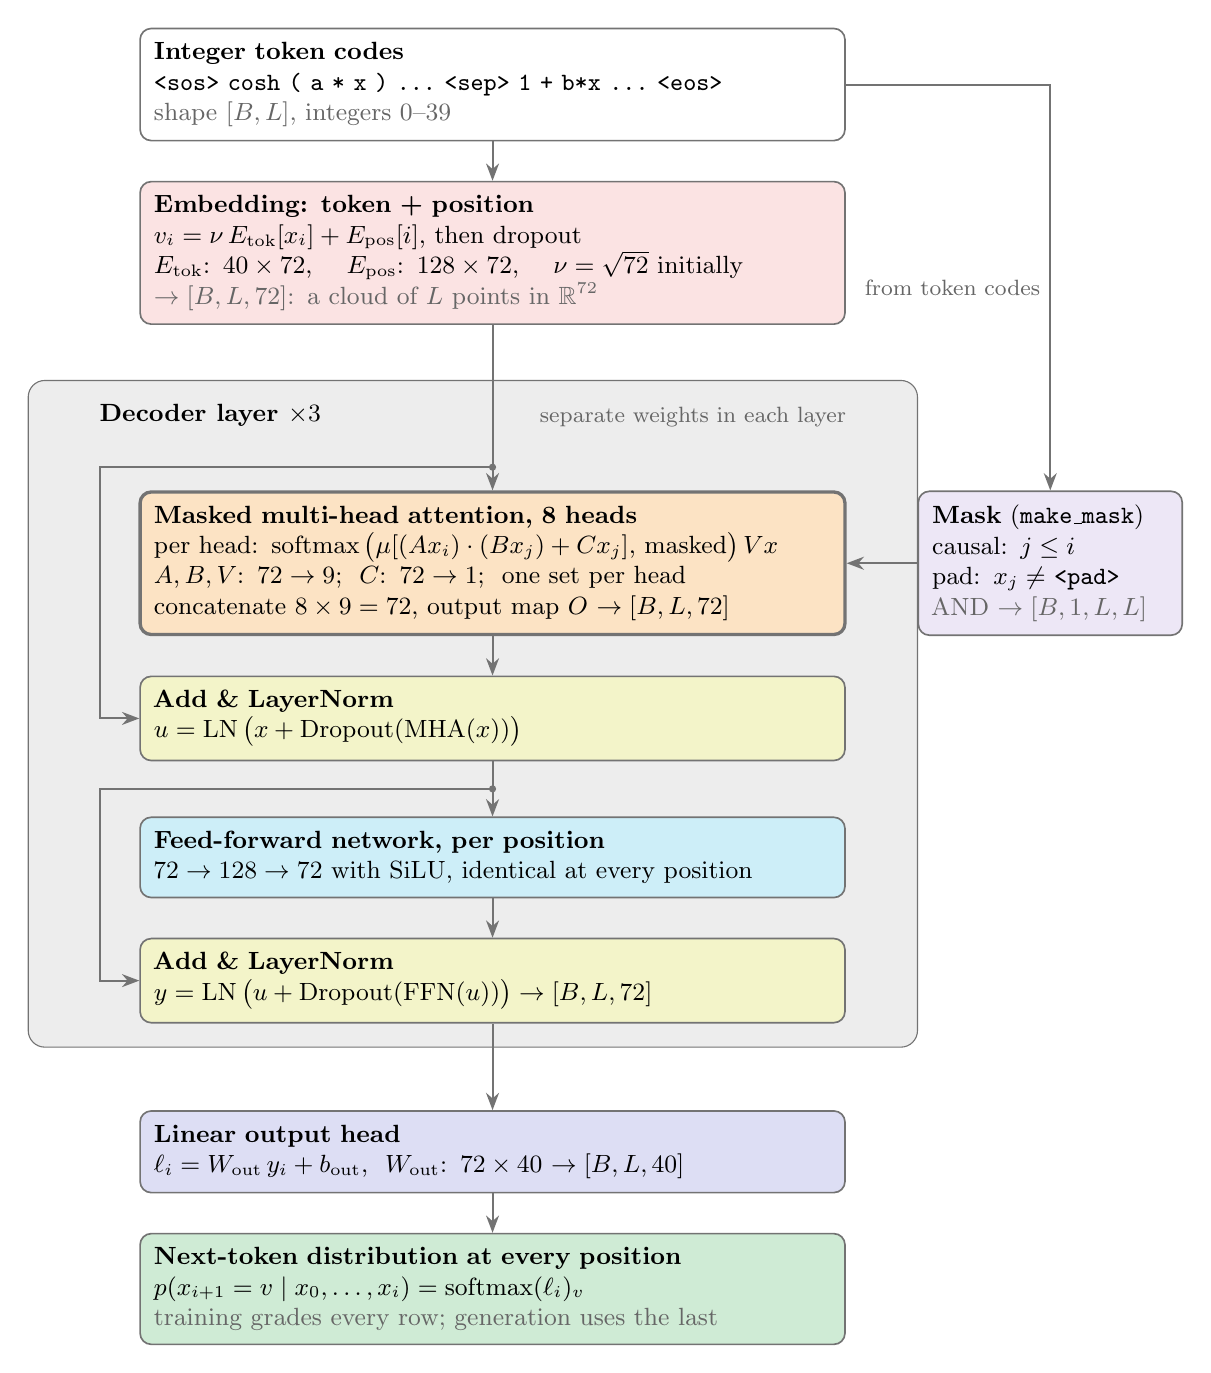
\begin{tikzpicture}[node distance=5mm]
  \def\bw{8.6cm}
  \node[blk,text width=\bw] (in) {\textbf{Integer token codes}\\
    \code{<sos> cosh ( a * x ) \dots\ <sep> 1 + b*x \dots\ <eos>}\\
    {\color{black!60}shape $[B,L]$, integers 0--39}};
  \node[blk,fill=cEmb,text width=\bw,below=of in] (emb) {\textbf{Embedding: token + position}\\
    $v_i=\nu\,\Etok[x_i]+\Epos[i]$, then dropout\\
    $\Etok$: $40\times72$, \quad $\Epos$: $128\times72$, \quad $\nu=\sqrt{72}$ initially\\
    {\color{black!60}$\to[B,L,72]$: a cloud of $L$ points in $\R^{72}$}};
  \node[blk,fill=cAtt,line width=1.2pt,text width=\bw,below=21mm of emb] (attn) {\textbf{Masked multi-head attention, 8 heads}\\
    per head: $\softmax\big(\mu[(Ax_i)\cdot(Bx_j)+Cx_j]\text{, masked}\big)\,Vx$\\
    $A,B,V$: $72\to9$; \ $C$: $72\to1$; \ one set per head\\
    concatenate $8\times9=72$, output map $O$ $\to[B,L,72]$};
  \node[blk,fill=cNorm,text width=\bw,below=of attn] (add1) {\textbf{Add \& LayerNorm}\\
    $u=\LN\big(x+\mathrm{Dropout}(\mathrm{MHA}(x))\big)$};
  \node[blk,fill=cFF,text width=\bw,below=7mm of add1] (ffn) {\textbf{Feed-forward network, per position}\\
    $72\to128\to72$ with SiLU, identical at every position};
  \node[blk,fill=cNorm,text width=\bw,below=of ffn] (add2) {\textbf{Add \& LayerNorm}\\
    $y=\LN\big(u+\mathrm{Dropout}(\mathrm{FFN}(u))\big)\to[B,L,72]$};
  \node[blk,fill=cLin,text width=\bw,below=11mm of add2] (head) {\textbf{Linear output head}\\
    $\ell_i=W_{\text{out}}\,y_i+b_{\text{out}}$, \ $W_{\text{out}}$: $72\times40$ $\to[B,L,40]$};
  \node[blk,fill=cSoft,text width=\bw,below=of head] (dist) {\textbf{Next-token distribution at every position}\\
    $p(x_{i+1}=v\mid x_0,\dots,x_i)=\softmax(\ell_i)_v$\\
    {\color{black!60}training grades every row; generation uses the last}};
  \node[blk,fill=cMask,text width=3.0cm,right=9mm of attn] (mask) {\textbf{Mask} (\code{make\_mask})\\
    causal: $j\le i$\\
    pad: $x_j\neq$ \tok{pad}\\
    {\color{black!60}AND $\to[B,1,L,L]$}};

  % container for one decoder layer
  \node[anchor=south west,font=\small\bfseries,inner sep=0pt] (lbl) at ($(attn.north west)+(-5mm,8mm)$) {Decoder layer $\times3$};
  \node[anchor=south east,note,inner sep=0pt] at ($(attn.north east)+(0,8mm)$) {separate weights in each layer};
  \begin{scope}[on background layer]
    \node[draw=edge,fill=tint,rounded corners=6pt,inner xsep=9mm,inner ysep=3mm,
          fit=(lbl)(attn)(add2)] (stack) {};
  \end{scope}

  % main flow
  \draw[flow] (in) -- (emb);
  \draw[flow] (emb) -- coordinate[pos=0.86] (tap1) (attn);
  \draw[flow] (attn) -- (add1);
  \draw[flow] (add1) -- coordinate[pos=0.5] (tap2) (ffn);
  \draw[flow] (ffn) -- (add2);
  \draw[flow] (add2) -- (head);
  \draw[flow] (head) -- (dist);
  % residual paths
  \fill[edge] (tap1) circle (1.3pt);
  \fill[edge] (tap2) circle (1.3pt);
  \draw[flow] (tap1) -| ($(add1.west)+(-5mm,0)$) -- (add1.west);
  \draw[flow] (tap2) -| ($(add2.west)+(-5mm,0)$) -- (add2.west);
  % mask
  \draw[flow] (in.east) -| node[note,pos=0.75,left] {from token codes} (mask.north);
  \draw[flow] (mask.west) -- (attn.east);
\end{tikzpicture}
\caption{The tiny language model. Attention (orange) is the only step
  in which positions exchange information. Shapes are given for batch size $B$ and
  sequence length $L$.}
\label{fig:arch}
\end{figure}

% ==================================================================
\section{The components, one at a time}
% ==================================================================

Each subsection gives the mathematics, the tensor shapes, and the class in the
notebook that implements it, following the data through the model.

\subsection{Embedding: tokens and positions become points (\code{Decoder})}

Two learned lookup tables do the embedding: a token table $\Etok$ of shape
$40\times72$ and a position table $\Epos$ of shape $128\times72$ (both
\code{nn.Embedding}). The token $x_i$ at position $i$ becomes the vector
\begin{equation}
  v_i=\nu\,\Etok[x_i]+\Epos[i]\in\R^{72},
\end{equation}
where $\nu$ is a trainable scalar initialized to $\sqrt{72}\approx8.49$. Dropout is
applied to $v$, and the result has shape $[B,L,72]$: the sequence is now a cloud of
$L$ points in $\R^{72}$. In the notebook's geometric language, the token vector $t$
and the position vector $z$ span a line, and $v=\nu t+z$ is a point on it.

The position term is essential. Attention, defined below, treats its input as an
unordered set: permute the tokens and the outputs are permuted in the same way.
Without $\Epos$ the model could not tell \code{x**2/3} from \code{x**3/2}. The
positions here are \emph{learned} vectors, not the fixed sinusoids of Vaswani
\emph{et al.}

\subsection{Masks: who may look at whom (\code{TinyLM.make\_mask})}
\label{sec:mask}

The mask is a boolean array $M$ of shape $[B,1,L,L]$; the singleton axis lets one
mask serve all eight heads by broadcasting. Its entry for query position $i$ and key
position $j$ is
\begin{equation}
  M_{ij} = \underbrace{[\,j\le i\,]}_{\text{causal (\code{torch.tril})}}
     \;\wedge\; \underbrace{[\,x_j\neq\tok{pad}\,]}_{\text{pad}} .
\end{equation}
For the five-token sequence $\tok{sos},p,\tok{sep},t_1,\tok{eos}$ the causal part is
lower triangular (Figure~\ref{fig:mask}): row $i$ lists the positions that token $i$
may attend to.

\begin{figure}[h]
\centering
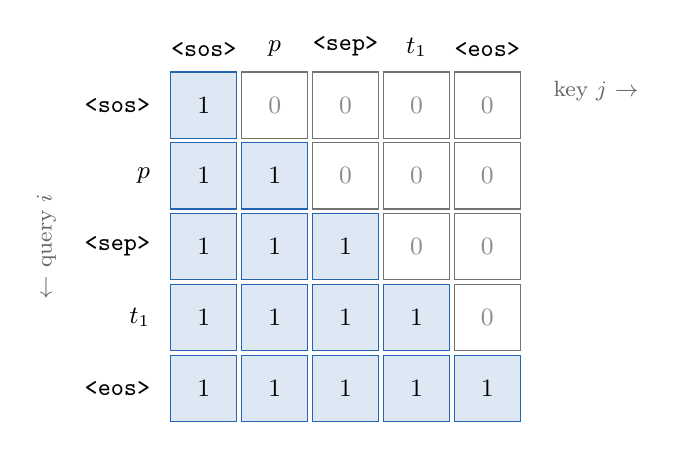
\begin{tikzpicture}[x=9mm,y=9mm]
  \foreach \lab [count=\i from 0] in {\tok{sos},$p$,\tok{sep},$t_1$,\tok{eos}} {
    \node[font=\small,anchor=east] at (-0.62,-\i) {\lab};
    \node[font=\small,anchor=south] at (\i,0.55) {\lab};
  }
  \foreach \i in {0,...,4} \foreach \j in {0,...,4} {
    \ifnum\j>\i
      \node[draw=edge,minimum size=8.4mm,font=\small\color{black!45}] at (\j,-\i) {0};
    \else
      \node[draw=accent,fill=accent!15,minimum size=8.4mm,font=\small] at (\j,-\i) {1};
    \fi
  }
  \node[font=\footnotesize\color{black!60},anchor=west] at (4.8,0.2) {key $j$ $\rightarrow$};
  \node[font=\footnotesize\color{black!60},rotate=90,anchor=south] at (-1.95,-2) {$\leftarrow$ query $i$};
\end{tikzpicture}
\caption{The causal mask for a five-token sequence. Row $i$ marks the tokens that
  token $i$ may attend to: itself and those before it.}
\label{fig:mask}
\end{figure}

Wherever $M_{ij}=0$ the attention score is overwritten with $-10^{10}$ before the
softmax, so its weight becomes exactly zero. The pad mask removes \emph{columns}
(pads cannot be looked at); it does not remove rows. With \code{PROMPT\_MASK = True}
the prompt block would be fully visible to itself (a ``prefix LM''); the notebook
keeps it \code{False}, so the prompt, too, is read strictly left to right.

\subsection{Attention: the $(A,B,C)$ parametrization (\code{AttentionHead}, \code{MultiHeadAttention})}

This is the heart of the model.

\paragraph{The textbook form.} With $Q=xA_Q^T+b_Q$, $K=xA_K^T+b_K$ and
$V=xA_V^T+b_V$, attention is $\softmax(\mu QK^T)V$. Expanding one score gives
\begin{equation}
  Q_iK_j^T = x_iA_Q^TA_K\,x_j^T + x_iA_Q^Tb_K^T + b_QA_K\,x_j^T + b_Qb_K^T .
\end{equation}

\paragraph{The symmetry of the softmax.} The softmax acts along the key index $j$ and
is unchanged when the same constant is added to every entry of a row. The second and
fourth terms do not depend on $j$, so they cancel: the key bias $b_K$ never affects an
attention weight. The third term survives, but it is a single fixed row vector,
$C\equiv b_QA_K$, dotted into each $x_j$, so it is given its own parameter.

\paragraph{The result.} Writing $A\equiv A_Q$ and $B\equiv A_K$ (both without bias),
head $\ell$ computes, for query position $i$,
\begin{align}
  S^{(\ell)}_{ij} &= \mu_\ell\big[(A_\ell x_i)\cdot(B_\ell x_j)+C_\ell x_j\big], \\
  w^{(\ell)}_{ij} &= \frac{M_{ij}\,e^{S^{(\ell)}_{ij}}}{\sum_{j'}M_{ij'}\,e^{S^{(\ell)}_{ij'}}}, \\
  \operatorname{head}_\ell(x)_i &= \sum_{j\le i} w^{(\ell)}_{ij}\,\big(V_\ell x_j+b_\ell\big),
\end{align}
with $A_\ell,B_\ell,V_\ell$ each $9\times72$, $C_\ell$ of size $1\times72$,
$b_\ell\in\R^9$, and $\mu_\ell$ a trainable scale initialized to $1/\sqrt9=1/3$.

Every textbook head is an $(A,B,C)$ head: take $C_\ell=b_{Q,\ell}A_{K,\ell}$. The
converse is not quite true. In the textbook form that linear term is confined to the
row space of $A_{K,\ell}$, of dimension at most 9, whereas $C_\ell$ may be any vector in
$\R^{72}$. The $(A,B,C)$ family is therefore slightly larger, and it no longer carries
the key bias, which cannot affect the output. A trained $Q/K/V$ model can be converted
into an $(A,B,C)$ model exactly, which is how the checkpoint in \code{runs/TLM\_ABC/}
was made. The three pieces have simple readings.

\begin{itemize}
\item \textbf{$A$ and $B$: a learned similarity.} $(A_\ell x_i)\cdot(B_\ell x_j) =
  x_i^TW_\ell x_j$ with $W_\ell=A_\ell^TB_\ell$, a $72\times72$ bilinear form of rank at
  most 9. Only $W_\ell$ is identifiable, so ``query'' and ``key'' are just names for its
  two low-rank factors.
\item \textbf{$C$: a prior on each key.} $C_\ell x_j$ depends on token $j$ alone. It
  says how attractive token $j$ is to every query, whatever the query is.
\item \textbf{The softmax: a convex combination.} Each row $w_{i\cdot}$ is non-negative
  and sums to one, so it is a point on the probability simplex. The head's output for
  token $i$ therefore lies in the convex hull of the value vectors of tokens
  $0,\dots,i$, and of nothing later.
\end{itemize}

The scale $\mu$ keeps the scores of order one. If the nine components of $A_\ell x$
and $B_\ell x$ have roughly unit variance, their dot product has variance about 9, and
multiplying by $1/3$ prevents the softmax from saturating early in training.

\paragraph{Many heads.} The eight heads act in parallel on the same input. Their
9-dimensional outputs are concatenated into one 72-vector and mixed by an output map
$O$ ($72\times72$ plus bias):
\begin{equation}
  \mathrm{MHA}(x)_i = O\big[\operatorname{head}_1(x)_i\,\|\,\cdots\,\|\,\operatorname{head}_8(x)_i\big]+b_O .
\end{equation}
One head offers one rank-9 notion of similarity; eight heads let a token gather eight
different kinds of context at once.

\paragraph{Two implementations, one function.} \code{MultiHeadAttentionPerHead} builds
each head as its own \code{AttentionHead} object and loops over them, so each head's
parameters are visible in the code. \code{MultiHeadAttention}, the version the model
uses, stacks the eight heads into single $72\times72$ layers and splits the result by
reshaping. For equal weights the outputs are identical; the fused version is faster
because a few large matrix products use a GPU far better than many small ones.
Table~\ref{tab:mha} traces its shapes.

\begin{table}[h]
\centering\small
\caption{Shape bookkeeping in \code{MultiHeadAttention.forward}.}
\label{tab:mha}
\begin{tabular}{@{}cll@{}}
\toprule
Step & Operation & Shape \\
\midrule
1 & $Ax$, $Bx$, $Vx$ & $[B,L,72]$ \\
2--3 & split into heads and permute & $[B,8,L,9]$ \\
4 & $S=Ax\,(Bx)^T$ & $[B,8,L,L]$ \\
5 & add $C(x)$ (permuted to $[B,8,1,L]$); multiply by $\mu$ (shape $[8,1,1]$) & $[B,8,L,L]$ \\
6 & mask with $-10^{10}$, softmax over keys, dropout & $[B,8,L,L]$ \\
7 & $W\,Vx$, then permute and merge heads & $[B,L,72]$ \\
8 & output layer $O$ & $[B,L,72]$ \\
\bottomrule
\end{tabular}
\end{table}

\paragraph{A remark on the value bias.} Within one head the value bias $b_\ell$ is not
removed by the softmax: because each row of weights sums to one, it is carried through
as a constant shift of the head's output. After concatenation, however, that shift
becomes the constant vector $O[b_1\|\cdots\|b_8]$, which the output bias $b_O$ can
absorb. At the level of the multi-head layer the value bias is therefore redundant
(216 of the 136{,}169 parameters); it is kept to stay close to the standard form.

\subsection{Feed-forward network (\code{Feedforward})}

After attention has mixed information \emph{between} tokens, a small two-layer
network processes each token \emph{on its own}, with the same weights at every
position:
\begin{equation}
  \mathrm{FFN}(u) = W_2\,\mathrm{Dropout}\big(\mathrm{SiLU}(W_1u+b_1)\big)+b_2,
  \qquad \mathrm{SiLU}(z)=z\,\sigma(z),
\end{equation}
with $W_1:\R^{72}\to\R^{128}$ and $W_2:\R^{128}\to\R^{72}$. The dichotomy is worth
stating plainly: attention is the \emph{only} place where tokens communicate; the
feed-forward network is where each token processes what it has gathered.

\subsection{Residual connections and layer normalization (\code{DecoderLayer})}

A decoder layer wraps each of its two sub-layers in a residual connection followed by
layer normalization:
\begin{equation}
  u=\LN_1\big(x+\mathrm{Dropout}(\mathrm{MHA}(x))\big),\qquad
  y=\LN_2\big(u+\mathrm{Dropout}(\mathrm{FFN}(u))\big).
\end{equation}
In the residual form each sub-layer learns a \emph{correction} to its input rather than
a replacement, which is what makes stacks of layers trainable. Layer normalization
standardizes the 72 components of each token separately,
\begin{equation}
  \LN(z)=\gamma\odot\frac{z-\operatorname{mean}(z)}{\sqrt{\operatorname{var}(z)+10^{-5}}}+\beta,
  \qquad \gamma,\beta\in\R^{72}\ \text{learned}.
\end{equation}
Placing the normalization after the addition (``post-LN'') follows the original 2017
paper. A layer maps $[B,L,72]$ to $[B,L,72]$, so identical layers can be stacked.

\subsection{The output head (\code{Decoder.linear})}

A final linear map turns each 72-vector $y_i$ into 40 logits, one per vocabulary token:
\begin{equation}
  \ell_i=W_{\text{out}}\,y_i+b_{\text{out}}\in\R^{40},\qquad
  p(x_{i+1}=v\mid x_0,\dots,x_i)=\frac{e^{\ell_{i,v}}}{\sum_{u\in\V}e^{\ell_{i,u}}} .
\end{equation}
The output has shape $[B,L,40]$. Because of the causal mask, row $i$ depends only on
$x_0,\dots,x_i$, so every row is a legitimate next-token prediction for its own
prefix. One forward pass therefore yields $L$ predictions, a fact that both training
and generation exploit.

\subsection{Where the parameters live}

\begin{table}[h]
\centering\small
\caption{Parameter budget. The total matches the count printed by the notebook.}
\label{tab:params}
\begin{tabular}{@{}lr@{}}
\toprule
Component & Parameters \\
\midrule
Token embedding, $40\times72$ & 2{,}880 \\
Position embedding, $128\times72$ & 9{,}216 \\
Embedding scale $\nu$ & 1 \\
One layer: attention ($A,B$: 5{,}184 each; $C$: 576; $V,O$: 5{,}256 each; $\mu$: 8) & 21{,}464 \\
One layer: feed-forward ($9{,}344+9{,}288$) & 18{,}632 \\
One layer: two LayerNorms & 288 \\
\textbf{Three decoder layers} ($3\times40{,}384$) & \textbf{121{,}152} \\
Output head, $72\times40+40$ & 2{,}920 \\
\midrule
\textbf{Total} & \textbf{136{,}169} \\
\bottomrule
\end{tabular}
\end{table}

\noindent The three decoder layers hold 89\% of the parameters.

% ==================================================================
\section{Training: 127 predictions from one forward pass}
% ==================================================================

During training the model is fed the \emph{true} sequence and, thanks to the causal
mask, predicts the next token at every position simultaneously. Feeding the ground
truth rather than the model's own guesses is called \textbf{teacher forcing}. It is
what makes transformers much cheaper to train than recurrent networks, which must step
through a sequence one token at a time.

\subsection{Aligning predictions with targets (\code{TLMObjective.forward})}

Logit row $i$ predicts token $i+1$, so the two tensors are shifted by one before they
are compared: \code{logits[:, :-1, :]} drops the last row, because there is no token
after the last position to predict, and \code{sequence[:, 1:]} drops \tok{sos}, because nothing predicts it.
Both then have 127 positions, and the loss at each is the cross entropy
\begin{equation}
  \mathrm{loss}_i=-\log\frac{e^{\ell_{i,x_{i+1}}}}{\sum_{u\in\V}e^{\ell_{i,u}}} .
\end{equation}

\subsection{Which predictions are graded (\code{TinyLM.make\_loss\_mask})}

The model is graded only on the answer, not on the prompt. A loss mask keeps the
prediction made at position $i$ when $i$ is at or after \tok{sep} and its \emph{target}
$x_{i+1}$ is a real token, that is, an answer token or the \tok{eos} that ends the
answer. The empirical risk is the mean loss over the kept predictions:
\begin{equation}
  m_i=[\,i\ge i_{\text{sep}}\,]\wedge[\,x_{i+1}\neq\tok{pad}\,],\qquad
  R=\frac{\sum_{b,i}m_{b,i}\,\mathrm{loss}_{b,i}}{\sum_{b,i}m_{b,i}} .
\end{equation}
For the example of Table~\ref{tab:layout} this gives Table~\ref{tab:graded}.

\begin{table}[h]
\centering\small
\caption{Which predictions enter the loss for the example sequence.}
\label{tab:graded}
\begin{tabular}{@{}llll@{}}
\toprule
Input position & Input token & Target token & Graded? \\
\midrule
0--15 & \tok{sos} and prompt & prompt and \tok{sep} & no \\
16 & \tok{sep} & $t_1=$ \code{1} & yes \\
17--69 & $t_1,\dots,t_{53}$ & $t_2,\dots,t_{54}$ & yes \\
70 & $t_{54}=$ \code{O(x**6)} & \tok{eos} & yes \\
71 & \tok{eos} & \tok{pad} & no \\
72--126 & \tok{pad} & \tok{pad} & no \\
\bottomrule
\end{tabular}
\end{table}

The model is thus graded on 55 predictions: the 54 answer tokens, plus the \tok{eos}
that ends the answer. Note that the mask is defined by the \emph{target}. A mask defined
by the input alone (keep $i$ if $x_i\neq\tok{pad}$) would also grade the meaningless
prediction made at \tok{eos}, whose target is \tok{pad}.

\subsection{Optimization}

\begin{itemize}
\item Adam, with the gradient norm clipped at 1.
\item $8\times10^5$ iterations of batch 32, so each of the 12{,}000 training sequences is
  seen about 2{,}100 times.
\item Learning rate $1.6\times10^{-3}$, multiplied by $\gamma=0.831$ every 50{,}000
  iterations, ending at $1.0\times10^{-4}$.
\item Dropout ($p=0.1$) is active in \code{train()} mode and switched off in
  \code{eval()} mode, which is used for monitoring and generation.
\item Every 100 iterations the monitor evaluates the risk on 156 training and 156
  validation sequences and saves the parameters when the validation risk improves.
\end{itemize}

% ==================================================================
\section{Autoregressive generation}
\label{sec:generation}
% ==================================================================

At inference time the model is run once per output token: the last row of logits picks
the next token, which is appended to the input and fed back in (Figure~\ref{fig:gen}).
Nothing in the network changes between training and generation; only the way it is
called does.

\begin{figure}[t]
\centering
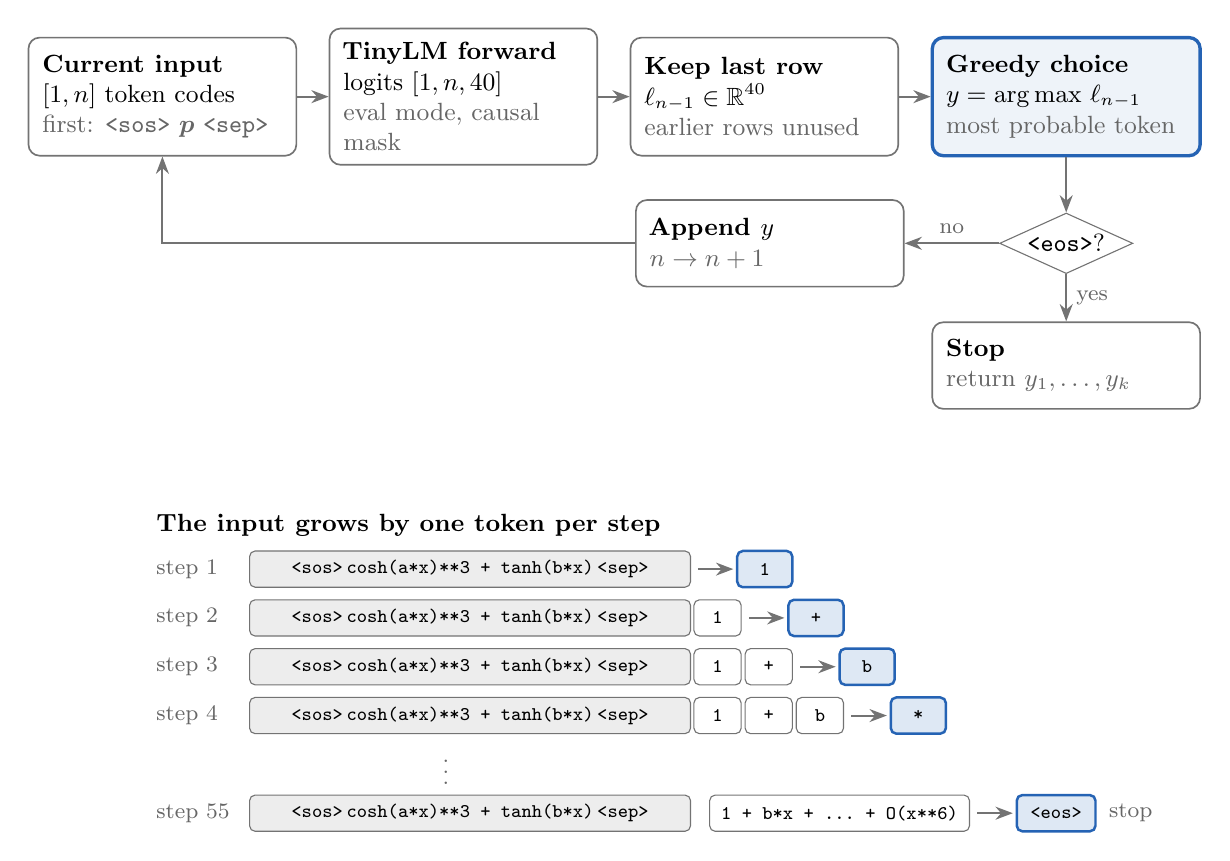
\begin{tikzpicture}[node distance=4mm]
  \tikzset{gb/.style={blk,align=flush left,text width=3.05cm,minimum height=15mm}}
  \node[gb] (seq) {\textbf{Current input}\\ $[1,n]$ token codes\\ {\color{black!60}first: \tok{sos} $\bm{p}$ \tok{sep}}};
  \node[gb,right=of seq] (fwd) {\textbf{TinyLM forward}\\ logits $[1,n,40]$\\ {\color{black!60}eval mode, causal mask}};
  \node[gb,right=of fwd] (last) {\textbf{Keep last row}\\ $\ell_{n-1}\in\R^{40}$\\ {\color{black!60}earlier rows unused}};
  \node[gb,hl,align=flush left,text width=3.05cm,minimum height=15mm,right=of last] (amax) {\textbf{Greedy choice}\\ $y=\arg\max\,\ell_{n-1}$\\ {\color{black!60}most probable token}};
  \node[diamond,draw=edge,aspect=2.2,inner sep=1pt,font=\small,below=7mm of amax] (dec) {\tok{eos}?};
  \node[gb,minimum height=11mm,left=12mm of dec] (app) {\textbf{Append $y$}\\ {\color{black!60}$n\to n+1$}};
  \node[gb,minimum height=11mm,below=6mm of dec] (stop) {\textbf{Stop}\\ {\color{black!60}return $y_1,\dots,y_k$}};
  \draw[flow] (seq) -- (fwd);
  \draw[flow] (fwd) -- (last);
  \draw[flow] (last) -- (amax);
  \draw[flow] (amax) -- (dec);
  \draw[flow] (dec) -- node[note,above] {no} (app);
  \draw[flow] (dec) -- node[note,right] {yes} (stop);
  \draw[flow] (app.west) -| (seq.south);

  % growing input
  \begin{scope}[yshift=-6.0cm,x=1cm,y=-0.62cm]
    \node[font=\small\bfseries,anchor=west] at (-0.2,-0.9) {The input grows by one token per step};
    \tikzset{pc/.style={draw=edge,fill=tint,rounded corners=2pt,minimum height=4.6mm,inner sep=1pt,font=\scriptsize},
             gc/.style={draw=edge,rounded corners=2pt,minimum height=4.6mm,minimum width=6mm,inner sep=1pt,font=\scriptsize},
             yc/.style={draw=accent,fill=accent!15,line width=0.9pt,rounded corners=2pt,minimum height=4.6mm,minimum width=7mm,inner sep=1pt,font=\scriptsize\bfseries}}
    \newcommand{\prompt}[1]{\node[pc,anchor=west,minimum width=5.6cm] at (1.1,#1) {\tok{sos}\,\code{cosh(a*x)**3 + tanh(b*x)}\,\tok{sep}};}
    \foreach \r/\lab in {0/step 1,1/step 2,2/step 3,3/step 4} {\node[note,anchor=west] at (-0.2,\r) {\lab}; \prompt{\r}}
    \node[note,anchor=west] at (-0.2,5) {step 55};
    \prompt{5}
    \node[note] at (3.6,4) {$\vdots$};
    % generated tokens
    \node[gc] at (7.05,1) {\code{1}};
    \node[gc] at (7.05,2) {\code{1}}; \node[gc] at (7.7,2) {\code{+}};
    \node[gc] at (7.05,3) {\code{1}}; \node[gc] at (7.7,3) {\code{+}}; \node[gc] at (8.35,3) {\code{b}};
    \node[gc,minimum width=3.3cm] at (8.6,5) {\code{1 + b*x + \dots\ + O(x**6)}};
    % predictions
    \draw[flow] (6.8,0) -- (7.25,0); \node[yc] at (7.65,0) {\code{1}};
    \draw[flow] (7.45,1) -- (7.9,1); \node[yc] at (8.3,1) {\code{+}};
    \draw[flow] (8.1,2) -- (8.55,2); \node[yc] at (8.95,2) {\code{b}};
    \draw[flow] (8.75,3) -- (9.2,3); \node[yc] at (9.6,3) {\code{*}};
    \draw[flow] (10.35,5) -- (10.8,5); \node[yc,minimum width=10mm] at (11.35,5) {\tok{eos}};
    \node[note,anchor=west] at (11.9,5) {stop};
  \end{scope}
\end{tikzpicture}
\caption{Greedy autoregressive generation (\code{greedy\_generate}). Top: one iteration
  of the loop. Bottom: the input for the example of Table~\ref{tab:layout}; shaded is the
  delimited prompt, highlighted the token predicted at each step, which becomes input
  at the next step.}
\label{fig:gen}
\end{figure}

\subsection{The algorithm (\code{greedy\_generate})}

\begin{enumerate}
\item \textbf{Start} with the delimited prompt $s=\tok{sos},p_1,\dots,p_m,\tok{sep}$, of
  shape $[1,m+2]$; \code{seqdata.split} cuts it from a test sequence.
\item \textbf{Run the model} on $s$ in \code{eval()} mode, so that dropout is off, with
  the same causal mask as in training. The output has shape $[1,n,40]$ for the current
  length $n$.
\item \textbf{Keep only the last row} $\ell_{n-1}$. By the causal mask it depends on all
  of $s$ and on nothing else, so it defines the distribution of the next token given
  everything so far.
\item \textbf{Choose greedily}: $y=\arg\max_v\ell_{n-1,v}$.
\item \textbf{Stop or append.} If $y$ is \tok{eos}, stop. Otherwise append $y$, so that
  $n\to n+1$, and return to step 2. The loop runs at most $128-(m+2)$ times. (The code
  also stops on \tok{pad}, a safeguard for models trained before \tok{eos} was placed
  directly after the answer.)
\end{enumerate}

\subsection{What the loop computes}

The network defines the probability of a complete answer as a product of next-token
factors, each conditioned on the prompt and on the answer so far:
\begin{equation}
  p(t_1,\dots,t_k\mid\bm{p})=\prod_{i=1}^{k}
  p\big(t_i\,\big|\,\tok{sos},\bm{p},\tok{sep},t_1,\dots,t_{i-1}\big).
\end{equation}
Greedy decoding maximizes each factor in turn, which does not guarantee the largest
product: an early, locally best token can lead to a worse sequence overall. Beam search
(Section~\ref{sec:beam}) explores more of the space. For this deterministic task greedy
decoding already succeeds on $99.3\%\pm0.3\%$ of the 800 test functions, where the
uncertainty is the binomial $\sqrt{F(1-F)/N}$.

\subsection{Beam search (\code{beam\_generate})}
\label{sec:beam}

Beam search keeps the $W$ most probable partial answers, called \emph{beams}, instead of
only one; the notebook uses $W=5$. A beam's score is the log-probability of its partial
answer, $\log P(t_1,\dots,t_i\mid\bm{p})=\sum_{r\le i}\log p(t_r\mid\dots)$, so extending a
beam by the token $v$ simply adds $\log p(v\mid\text{beam})$ to its score.
Figure~\ref{fig:beam} shows one step of the loop and a small example with $W=2$.

\begin{figure}[t]
\centering
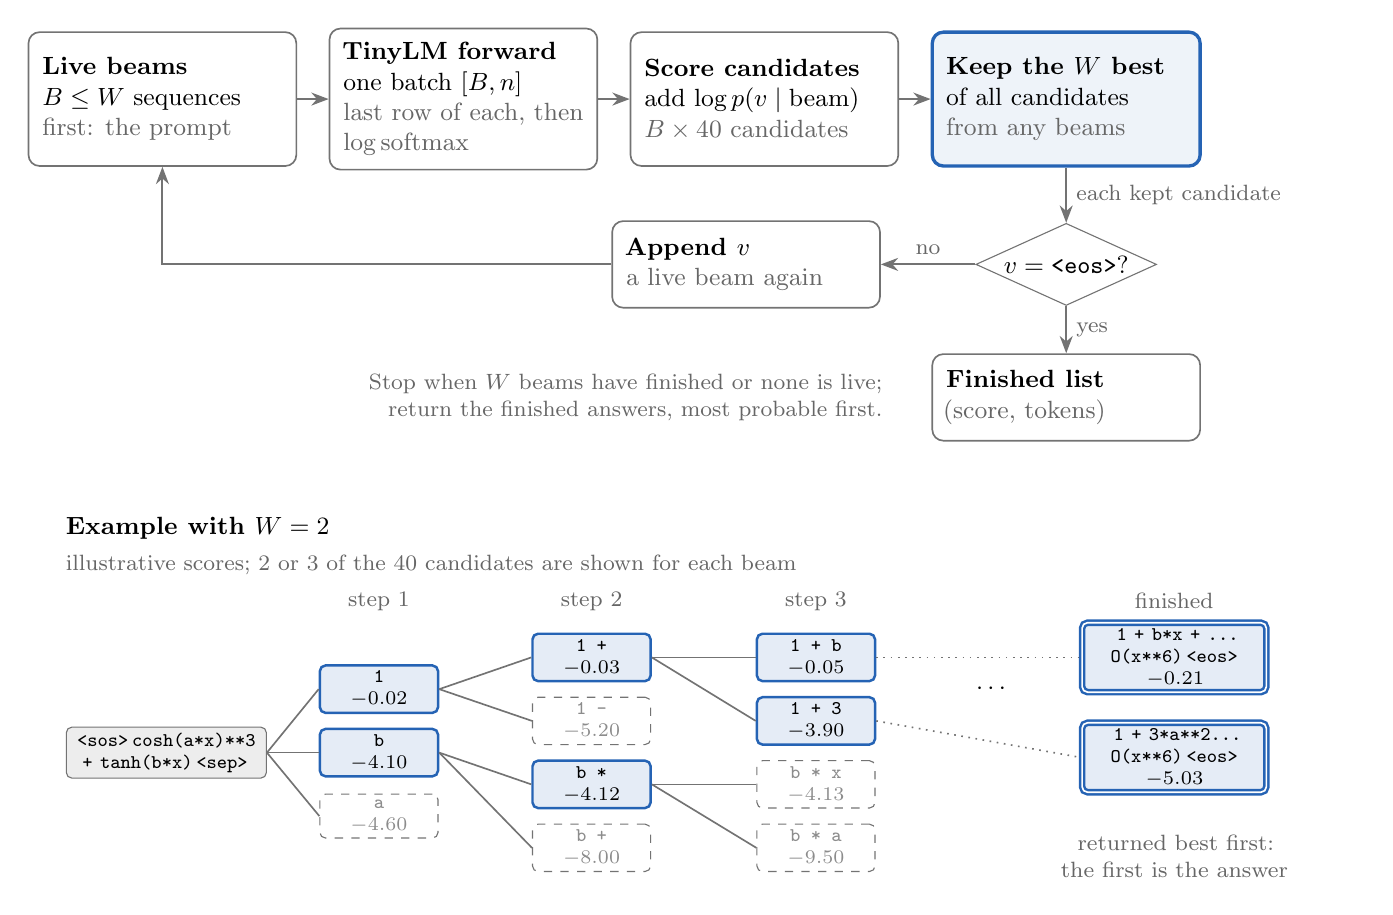
\begin{tikzpicture}[node distance=4mm]
  \tikzset{gb/.style={blk,align=flush left,text width=3.05cm,minimum height=17mm}}
  \node[gb] (live) {\textbf{Live beams}\\ $B\le W$ sequences\\ {\color{black!60}first: the prompt}};
  \node[gb,right=of live] (fwd) {\textbf{TinyLM forward}\\ one batch $[B,n]$\\ {\color{black!60}last row of each, then $\log\operatorname{softmax}$}};
  \node[gb,right=of fwd] (cand) {\textbf{Score candidates}\\ add $\log p(v\mid\text{beam})$\\ {\color{black!60}$B\times40$ candidates}};
  \node[gb,hl,align=flush left,text width=3.05cm,minimum height=17mm,right=of cand] (keep) {\textbf{Keep the $W$ best}\\ of all candidates\\ {\color{black!60}from any beams}};
  \node[diamond,draw=edge,aspect=2.2,inner sep=1pt,font=\small,below=7mm of keep] (dec) {$v=\tok{eos}$?};
  \node[gb,minimum height=11mm,left=12mm of dec] (app) {\textbf{Append $v$}\\ {\color{black!60}a live beam again}};
  \node[gb,minimum height=11mm,below=6mm of dec] (fin) {\textbf{Finished list}\\ {\color{black!60}(score, tokens)}};
  \node[note,anchor=east,align=right] at ($(fin.west)+(-5mm,0)$) {Stop when $W$ beams have finished or none is live;\\ return the finished answers, most probable first.};
  \draw[flow] (live) -- (fwd);
  \draw[flow] (fwd) -- (cand);
  \draw[flow] (cand) -- (keep);
  \draw[flow] (keep) -- node[note,right] {each kept candidate} (dec);
  \draw[flow] (dec) -- node[note,above] {no} (app);
  \draw[flow] (dec) -- node[note,right] {yes} (fin);
  \draw[flow] (app.west) -| (live.south);

  % example tree, W = 2
  \begin{scope}[yshift=-8.3cm,x=1cm,y=0.62cm]
    \tikzset{
      bn/.style={draw=edge,rounded corners=2pt,align=center,inner sep=2pt,font=\scriptsize,minimum width=15mm},
      kept/.style={bn,draw=accent,fill=accent!12,line width=0.9pt},
      drop/.style={bn,dashed,text=black!45},
      done/.style={bn,draw=accent,fill=accent!12,line width=0.9pt,double},
      tl/.style={draw=edge,line width=0.6pt},
    }
    \node[font=\small\bfseries,anchor=west] at (-1.35,4.6) {Example with $W=2$};
    \node[note,anchor=west] at (-1.35,3.85) {illustrative scores; 2 or 3 of the 40 candidates are shown for each beam};
    \foreach \x/\lab in {2.75/step 1,5.45/step 2,8.3/step 3,12.85/finished} \node[note] at (\x,3.1) {\lab};
    \node[bn,fill=tint,text width=24mm] (P) at (0.05,0) {\tok{sos}\,\code{cosh(a*x)**3}\\\code{+ tanh(b*x)}\,\tok{sep}};
    % step 1
    \node[kept] (a1) at (2.75,1.3)  {\code{1}\\ $-0.02$};
    \node[kept] (a2) at (2.75,0)    {\code{b}\\ $-4.10$};
    \node[drop] (a3) at (2.75,-1.3) {\code{a}\\ $-4.60$};
    \foreach \c in {a1,a2,a3} \draw[tl] (P.east) -- (\c.west);
    % step 2
    \node[kept] (b1) at (5.45,1.95)  {\code{1 +}\\ $-0.03$};
    \node[drop] (b2) at (5.45,0.65)  {\code{1 -}\\ $-5.20$};
    \node[kept] (b3) at (5.45,-0.65) {\code{b *}\\ $-4.12$};
    \node[drop] (b4) at (5.45,-1.95) {\code{b +}\\ $-8.00$};
    \draw[tl] (a1.east) -- (b1.west); \draw[tl] (a1.east) -- (b2.west);
    \draw[tl] (a2.east) -- (b3.west); \draw[tl] (a2.east) -- (b4.west);
    % step 3
    \node[kept] (c1) at (8.3,1.95)  {\code{1 + b}\\ $-0.05$};
    \node[kept] (c2) at (8.3,0.65)  {\code{1 + 3}\\ $-3.90$};
    \node[drop] (c3) at (8.3,-0.65) {\code{b * x}\\ $-4.13$};
    \node[drop] (c4) at (8.3,-1.95) {\code{b * a}\\ $-9.50$};
    \draw[tl] (b1.east) -- (c1.west); \draw[tl] (b1.east) -- (c2.west);
    \draw[tl] (b3.east) -- (c3.west); \draw[tl] (b3.east) -- (c4.west);
    % later steps
    \node[font=\small] at (10.55,1.3) {$\cdots$};
    \node[done,text width=22mm] (d1) at (12.85,1.95) {\code{1 + b*x + \dots}\\\code{O(x**6)}\,\tok{eos}\\ $-0.21$};
    \node[done,text width=22mm] (d2) at (12.85,-0.1) {\code{1 + 3*a**2\dots}\\\code{O(x**6)}\,\tok{eos}\\ $-5.03$};
    \draw[tl,dotted] (c1.east) -- (d1.west); \draw[tl,dotted] (c2.east) -- (d2.west);
    \node[note,anchor=north,text width=4.6cm,align=center] at (12.85,-1.5) {returned best first: the first is the answer};
  \end{scope}
\end{tikzpicture}
\caption{Beam search (\code{beam\_generate}). Top: one step of the loop. Bottom: an
  example with $W=2$ for the prompt of Table~\ref{tab:layout}. Highlighted beams are the
  $W$ best of \emph{all} candidates at that step; dashed ones are dropped. At step 3 both
  survivors descend from \code{1 +}, while \code{b *} leaves no child. Numbers are
  log-probabilities of the partial answers and are illustrative.}
\label{fig:beam}
\end{figure}

\noindent The loop in the code is as follows.
\begin{enumerate}
\item \textbf{Start} with a single live beam, the delimited prompt, with score 0, and an
  empty list of finished answers.
\item \textbf{Run the model once on all live beams.} They all have the same length $n$, so
  they form one batch of shape $[B,n]$ with $B\le W$. The last row of logits of each beam
  gives, through a log-softmax, $\log p(v\mid\text{beam})$ for all 40 tokens $v$.
\item \textbf{Score every candidate}, $S(\text{beam},v)=\log P(\text{beam})+\log
  p(v\mid\text{beam})$: $B\times40$ numbers.
\item \textbf{Keep the $W$ largest} of these, whichever beams they come from. A strong beam
  may keep several children and a weak one none.
\item \textbf{Sort the kept candidates.} One whose token $v$ is \tok{eos} is finished: its
  answer (without \tok{eos}) and score go to the finished list. The others are extended by
  $v$ and become the live beams of the next step.
\item \textbf{Stop} when the finished list holds $W$ answers, when no beam is live, or at
  the length limit. Return the finished answers sorted by score, most probable first.
\end{enumerate}

Four properties follow directly from the code.
\begin{itemize}
\item \textbf{$W=1$ is greedy decoding.} With one beam, the best candidate is the
  arg max of $\log p(v\mid\text{beam})$, the greedy token.
\item \textbf{Cost.} Each step is one forward pass on a batch of at most $W$ sequences:
  roughly $W$ times the arithmetic of greedy decoding, for the same number of steps.
\item \textbf{A pruned search.} A candidate dropped at one step is gone for good, so beam
  search is still a heuristic. It usually finds a more probable answer than greedy
  decoding, but neither is guaranteed to find the most probable one.
\item \textbf{No length normalization.} Every token adds $\log p\le0$ to the score, so,
  among finished answers, shorter ones are favored. Many implementations divide the score
  by a power of the length. Here the length of the answer is fixed by the function, so the
  effect is small.
\end{itemize}

\begin{table}[h]
\centering\small
\caption{Training and generation compared.}
\label{tab:traingen}
\begin{tabular}{@{}lll@{}}
\toprule
 & Training & Generation \\
\midrule
Input & the true sequence (teacher forcing) & the model's own previous outputs \\
Forward passes per sequence & 1 & one per output token (55 for the example) \\
Logit rows used & all 127, masked to the answer & only the last \\
Dropout & on & off \\
Causal mask & yes & yes \\
\bottomrule
\end{tabular}
\end{table}

\subsection{Why earlier positions need not be recomputed}

Because of the causal mask, appending a token at the end does not change the
computation for any earlier position: rows $0,\dots,n-1$ at step $n+1$ are identical to
rows $0,\dots,n-1$ at step $n$. \code{greedy\_generate} recomputes them anyway, so each
step repeats all the earlier work. Caching each layer's $Bx$, $Cx$ and $Vx$ for the past
tokens (a key/value cache) lets each step compute only the new row, which is how
production language models generate quickly.

% ==================================================================
\section{Beyond this model}
% ==================================================================

The tiny language model follows the 2017 design closely. Current language models differ
from it in a few ways that are easy to state.
\begin{itemize}
\item \textbf{Post-LN versus pre-LN.} This model normalizes after each residual addition,
  as in the 2017 paper. Most current language models normalize \emph{before} each
  sub-layer and add a final layer normalization, which trains more stably in deep stacks.
\item \textbf{Positions.} Learned absolute position vectors cap the length at 128. Modern
  models typically use relative schemes such as rotary embeddings (RoPE).
\item \textbf{Key/value cache.} Production models cache past keys and values, so that each
  generation step computes only one new row (Section~\ref{sec:generation}).
\item \textbf{Tied embeddings.} Here the output map $W_{\text{out}}$ is separate from the
  token table $\Etok$; many language models tie them.
\item \textbf{The end of the output is learned.} \tok{eos} is just another token, which
  the model learns to emit because it always follows the answer in the training data.
  Had the padding been placed before \tok{eos}, the model would have learned to end its
  output with \tok{pad} instead.
\end{itemize}

\section*{References}
\begin{enumerate}[label={[\arabic*]}]
\item A.~Vaswani \emph{et al.}, ``Attention is all you need,'' \emph{Advances in Neural
  Information Processing Systems} \textbf{30} (2017).
  \href{https://papers.nips.cc/paper/2017/file/3f5ee243547dee91fbd053c1c4a845aa-Paper.pdf}{NeurIPS proceedings}.
\item A.~Rush \emph{et al.}, ``The Annotated Transformer.''
  \href{https://nlp.seas.harvard.edu/annotated-transformer/}{nlp.seas.harvard.edu/annotated-transformer}.
\item J.~L.~Ba, J.~R.~Kiros and G.~E.~Hinton, ``Layer normalization,''
  arXiv:1607.06450 (2016).
\end{enumerate}

\end{document}
